\documentclass{article}
\usepackage{amssymb}
\usepackage{amsmath}
\usepackage{mathtools}
\usepackage{cancel}
\usepackage{tikz}
\newtheorem{theorem}{Theorem}
\newtheorem{definition}{Definition}
\newtheorem{corollary}{Corollary}
\newtheorem{proof}{Proof}

\DeclareMathOperator*{\argmin}{argmin}

\begin{document}
\title{Deriving the DFT}
\author{Anmol Parande}
\date{Spring 2019}
\maketitle
\section{The Fourier Series}
The Fourier Series tell us that any piecewise-continuous function $f(x)$ can be represented as a sum of sines and cosines.
$$f(t) = \frac{a_0}{2} + \sum_{n=1}^{\infty}{a_n cos(n\omega t)+b_n sin(n\omega t)}$$
Where
$$\omega = \frac{2\pi}{T}$$
$$a_n = \frac{2}{T}\int_{\frac{-T}{2}}^{\frac{T}{2}}{f(t)cos(n\omega t)}$$
$$b_n = \frac{2}{T}\int_{\frac{-T}{2}}^{\frac{T}{2}}{f(t)sin(n\omega t)}$$
$T$ is the length of the interval over which we are defining the Fourier Series for.\\\\
One way to think of the Fourier series is that we are "projecting" a function $f(x)$
onto the basis functions $sin(n\omega t)$ and $cos(n\omega t)$. In this perspective,
$a_n, b_n$ are simply the coefficients of the projection.\\\\
The Fourier series can also be written more compactly by expressing it in terms of complex numbers using Euler's formula.
$$2cos(n\omega t)=e^{j\omega t}+e^{-j\omega t}$$
$$2jcos(n\omega t)=e^{j\omega t}-e^{-j\omega t}$$
This gives us
$$\frac{a_0}{2} + \sum_{n=1}^{\infty}{a_n cos(n\omega t)+b_n sin(n\omega t)}$$
$$=\frac{a_0}{2} + \sum_{n=1}^{\infty}{\left[\frac{a_n}{2}(e^{jn\omega t}+e^{-jn\omega t})+\frac{b_n}{2j}(e^{jn\omega t}-e^{-jn\omega t})\right]}$$
$$=\frac{a_0}{2} + \sum_{n=1}^{\infty}{\left[(\frac{a_n}{2} + \frac{b_n}{2j})e^{jn\omega t}+(\frac{a_n}{2} - \frac{b_n}{2j})e^{-jn\omega t})\right]}$$
Notice that the two terms inside the sums are complex conjugates of each other.
This means we can compact this expression even more by changing the bounds of the summation to $(-\infty, \infty)$.
This gives us $$f(x) = \sum_{n=-\infty}^{\infty}{(\frac{a_n}{2} + \frac{b_n}{2j})e^{jn\omega t}}$$
If we now substitute our definitions for $a_n$ and $b_n$, we see
$$\frac{a_n}{2}+\frac{b_n}{2j} = \frac{2}{2T}\int_{\frac{-T}{2}}^{\frac{T}{2}}{f(x)(cos(n\omega t)-jsin(n\omega t)}$$ 
$$cos(n\omega t) - jsin(n \omega t) = e^{-jn\omega t}$$
$$\therefore \frac{a_n}{2}+\frac{b_n}{2j} = \frac{1}{T}\int_{\frac{-T}{2}}^{\frac{T}{2}}{f(x)e^{-jn\omega t}}$$
We'll call these coefficients $c_n$, and we can now write the Fourier Series for a function $f(x)$ in its complex form.
$$f(x) = \sum_{n=-\infty}^{\infty}{c_ne^{jn\omega t}}$$
\section{Discrete Fourier Transform}
The Discrete Fourier Transform is going to make use of the Fourier Series to "project"
our data onto a basis of sines and cosines. This means we have a set of $N$ points $x_0...x_{N-1}$
which are apart by interval $\Delta$.
\[
    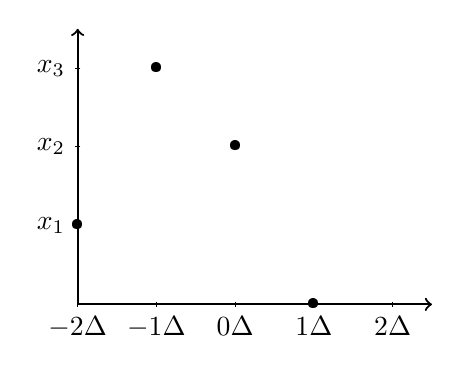
\begin{tikzpicture}
        \draw[thick,->] (0, 0) -- (4.5,0);
        \draw[thick,->] (0,0) -- (0,3.5);
        \foreach \x in {-2,-1, 0, 1, 2}
            \draw (\x+2,1pt) -- (\x + 2,-1pt) node[anchor=north] {$\x \Delta$};
        \foreach \y in {1,2,3}
            \draw (1pt,\y cm) -- (-1pt,\y cm) node[anchor=east] {$x_{\y}$};
        \foreach \Point in {(0,1), (2,2), (1,3), (3, 0)}{
            \node at \Point {\textbullet};
        }
    \end{tikzpicture}
\]
This can be represented as a vector 
\[
    \vec{x} = \left[
        \begin{array}{c}
            x_0\\
            x_1\\
            \vdots\\
            x_{N-1}
        \end{array}
    \right]
\]
Finding the Fourier Series requires a piecewise-continuous function, so lets perform zero-order hold interpolation
to get a function $x(t)$.
\[
    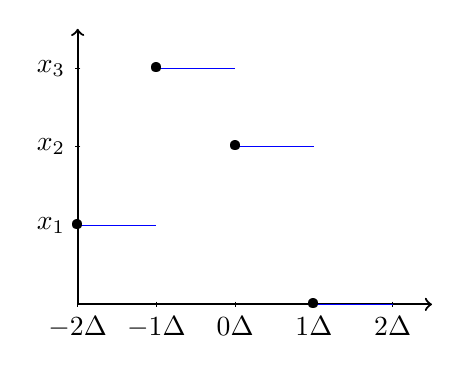
\begin{tikzpicture}
        \draw[thick,->] (0, 0) -- (4.5,0);
        \draw[thick,->] (0,0) -- (0,3.5);
        \foreach \x in {-2,-1, 0, 1, 2}
            \draw (\x+2,1pt) -- (\x + 2,-1pt) node[anchor=north] {$\x \Delta$};
        \foreach \y in {1,2,3}
            \draw (1pt,\y cm) -- (-1pt,\y cm) node[anchor=east] {$x_{\y}$};
        \draw[scale=1,domain=0:1,smooth,variable=\x,blue] plot ({\x},{1});
        \draw[scale=1,domain=2:3,smooth,variable=\x,blue] plot ({\x},{2});
        \draw[scale=1,domain=1:2,smooth,variable=\x,blue] plot ({\x},{3});
        \draw[scale=1,domain=3:4,smooth,variable=\x,blue] plot ({\x},{0});
        \foreach \Point in {(0,1), (2,2), (1,3), (3, 0)}{
            \node at \Point {\textbullet};
        }
    \end{tikzpicture}
\]
For example, our new function $x(t)$ might look something like above.
The other requirement of using the Fourier series is that we assume the 
function is periodic (i.e this signal will continue to repeat.). Our function 
has period $T = \Delta N$\\\\
To figure out what this function looks like in the basis of sines and cosines,
we need to find $c_n$.
$$c_n=\frac{1}{T}\int_{\frac{-T}{2}}^{\frac{T}{2}}{f(x)e^{-jn\omega t}}$$
Since our function is simply a bunch of lines, we can easily calculate the integral
by measuring the area under the curve.
$$c_n = \frac{\Delta}{T}\sum_{i=0}^{N-1}{x_i e^{-jn\omega i\Delta t}}$$
Using the fact that $T=\Delta n$ and $\omega = \frac{2\pi}{T}$, this simplifies To
$$c_n = \frac{1}{N}\sum_{i=0}^{N-1}{x_i e^{\frac{-jn 2\pi i}{N}}}$$
Notice that $\omega_N = e^{\frac{j2\pi}{N}}$ is the Nth root of unity. This gives us
$$c_n = \frac{1}{N}\sum_{i=0}^{N-1}{x_i \omega_N^{-ni}}$$
Writing out the full Fourier Series,
we see $$x(t) = \sum_{n=-\infty}^{\infty}{c_ne^{jn\omega t}} = \frac{1}{N}\sum_{n=-\infty}^{\infty}{\sum_{i=0}^{N-1}{x_i \omega_N^{-ni}}e^{jn\omega t}}$$
Because our signal only has $N$ samples, we only really care about $N$ terms of this series.
Specifically, we only care about the $c_n, n\in[0, N-1]$.
This means we can simplify this to $$x(t) = \sum_{n=-\infty}^{\infty}{c_ne^{jn\omega t}} \approx \frac{1}{N}\sum_{n=0}^{N-1}{\sum_{i=0}^{N-1}{x_i \omega_N^{-ni}}e^{jn\omega t}}$$
Remember that the original goal is to figure out how the vector $x(t)$, which represents our discrete signal,
is represented in terms of sines and cosines. Since we only care about the coefficients, we can write this sum as a matrix-vector product for the coefficients.
\[
    \left[
        \begin{array}{cccc}
            \omega_N^{-0*0} & \omega_N^{-0*1} & ... & \omega_N^{-0*(N-1)}\\
            \omega_N^{-1*0} & \ddots & & \vdots\\
            \vdots & & \ddots &\\
            \omega_N^{-(N-1)*0} & ... & & \omega_N^{-(N-1)(N-1)} 
    
        \end{array}
    \right]\left[
        \begin{array}{c}
            x_0\\
            x_1\\
            \vdots\\
            x_{N-1}
        \end{array}
    \right]
\]
The matrix on the left is the DFT matrix that we wanted.
The result of the product are the coefficients of our discrete signal 
in the DFT basis, a basis of sines and cosines.
\end{document}